%        File: TFGGuillermo.tex
%     Created: sáb mar 03 09:00  2018 C
% Last Change: sáb mar 03 09:00  2018 C
%
\documentclass[12pt,a4paper,twoside]{article}
\usepackage[utf8]{inputenc}
\usepackage[english, spanish, es-noquoting]{babel}
\usepackage[left=2.5cm,right=2.5cm,top=2.5cm,bottom=2.5cm]{geometry}
\usepackage{amsmath}
\usepackage{amsfonts}
\usepackage{amssymb}
\usepackage{amsthm, mathtools}
\usepackage{tikz,tikz-cd}
\usetikzlibrary{arrows, babel}
\usepackage{url}
\usepackage[colorlinks=true,linktocpage=true,pagebackref=true,linkcolor=blue]{hyperref}
\usepackage{remreset}
\usepackage{enumitem}
\usepackage{titlepic}
\usepackage{titlesec}
\usepackage{graphicx}
\usepackage{mathrsfs}
\usepackage{anyfontsize}
\usepackage{tocbibind}
\usepackage[tocflat]{tocstyle}
\usepackage{hyperref}
\usepackage{fancyhdr}
\usepackage[overload]{empheq}


\renewcommand{\thesection}{\arabic{section}}

%Otro formato para las secciones
\titleformat{\section}[block]
{\fontsize{15}{18}\bfseries\sffamily\filcenter}
{\S \thesection.}
{1em}
{}

\makeatletter
\@removefromreset{section}{chapter}
\makeatother

%Márgenes
%\voffset=-1.5cm
%\hoffset=-1.5cm
%\setlength{\textwidth}{16cm}
%\setlength{\textheight}{23cm}
%\setlength{\headsep}{25pt}
%\footskip=30pt

%\parskip=1.2ex

%\usepackage{bm} Para poner los vectores de otra forma

%Fuente Palatino:
%\usepackage[sc]{mathpazo}
%Fuente Times:
\usepackage{newtxtext}
\usepackage{newtxmath}
%Fuente Libertine:
%\usepackage{libertine}
%\usepackage[libertine]{newtxmath}

%Para probar texto ciego:
%\usepackage{blindtext}

\newtheorem{thm}{Teorema}[section]
\newtheorem{prop}[thm]{Proposición}
\newtheorem{lema}{Lema}
\newtheorem{corol}[thm]{Corolario}
\theoremstyle{definition} \newtheorem{defn}[thm]{Definición}
\theoremstyle{definition} \newtheorem{ejemplo}[thm]{Ejemplo}
\theoremstyle{definition} \newtheorem{ejercicio}[thm]{Ejercicio}
\theoremstyle{remark} \newtheorem*{obs}{Observación}


\def\CC{\mathbb{C}}
\def\QQ{\mathbb{Q}}
\def\ZZ{\mathbb{Z}}
\def\RR{\mathbb{R}}
\def\TT{\mathbb{T}}
\def\SF{\mathbb{S}}
\def\NN{\mathbb{N}}
\def\dd{\mathrm{d}}
\def\lie{\mathscr{L}}
\def\gg{\mathfrak{g}}
\def\zz{\bar{z}}

%\newcommand{\vect}[1]{\bm{#1}}
\newcommand{\vect}[1]{\mathbf{#1}}
%\newcommand{\vect}[1]{\vec{#1}}

\newcommand{\parcial}[2]{\frac{\partial #1}{\partial #2}}
\newcommand{\pois}[2]{\left\lbrace#1,#2\right\rbrace}

\title{TRABAJO DE FIN DE GRADO \\  Modelos superintegrables: El hamiltoniano de TTW}
\author{\bf Guillermo Gallego}
%\date{\bf \today}
\date{Junio 2018}

\pagestyle{fancy}
\fancyhf{}
\fancyhead[LE,RO]{\thepage}
\fancyhead[CO]{\small \sc MODELOS SUPERINTEGRABLES: EL HAMILTONIANO DE TTW}
\fancyhead[CE]{\small \sc GUILLERMO GALLEGO}
\renewcommand{\headrulewidth}{0pt}

\begin{document}
%\title[SIMETRÍAS EN MODELOS INTEGRABLES Y SUPERINTEGRABLES]{
%{\rm\tiny Trabajo  \hspace{-1mm}de  \hspace{-1mm}Fin  \hspace{-1mm}de  \hspace{-1mm}Grado,  
%\hspace{-1mm}Junio  \hspace{-1mm}2018}\\[8pt] 
%SIMETRÍAS EN MODELOS INTEGRABLES Y SUPERINTEGRABLES\\[8pt]
%{\rm\tiny Departamento \hspace{-1mm}de  \hspace{-1mm}Física  \hspace{-1mm}Teórica\\
%Facultad  \hspace{-1mm}de  \hspace{-1mm}Ciencias \hspace{-1mm}Físicas,  \hspace{-1mm}UCM\\
%{\rm\tiny Dirigido por Miguel A. Rodríguez}
%}}

\begin{titlepage}
%\vspace*{-2cm}
%\makebox[.5\textwidth][l]{\Large\bfseries\sffamily TRABAJO DE FIN DE GRADO \\ JUNIO 2018} 
%\makebox[.5\textwidth][r]{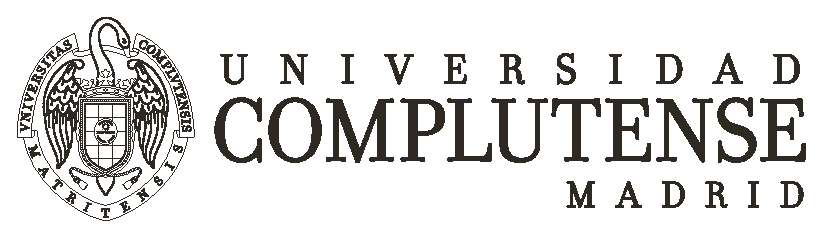
\includegraphics[height=1.5cm]{Negro-transparente}} 
%\makebox[\dimexpr\textwidth][r]{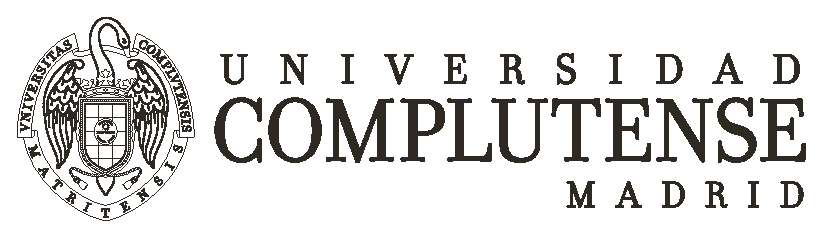
\includegraphics[height=1.5cm]{Negro-transparente}} 
\begin{minipage}{0.5\textwidth}
  \centering
    \Large TRABAJO DE FIN DE GRADO 
  \end{minipage}
\begin{minipage}{0.5\textwidth}
  \centering
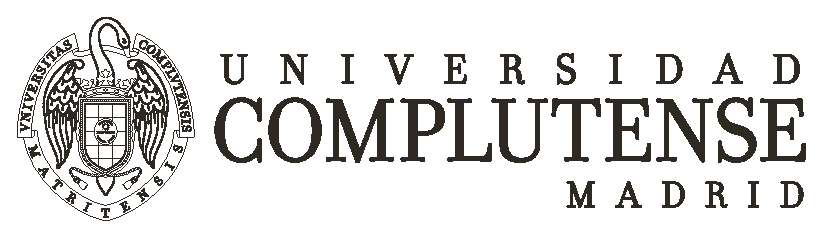
\includegraphics[height=1.5cm]{Negro-transparente}
  \end{minipage}

\vspace*{2cm}
\begin{center}
%\sc \large TRABAJO DE FIN DE GRADO, JUNIO 2018 \\
%\vspace*{.25 cm}
%    \today

%\vspace*{.5cm}
\rm \Huge\bfseries\sffamily Modelos superintegrables: el hamiltoniano de Tremblay-Turbiner-Winternitz

\vspace*{1cm}
\rm \normalsize \bfseries\sffamily Superintegrable models: the Tremblay-Turbiner-Winternitz hamiltonian

\vspace*{1cm}
\rm \large 
\sc GUILLERMO GALLEGO

\vspace*{.5 cm}
\sc \normalsize JUNIO 2018 \\
%    \today
\end{center}

\vspace*{2cm}

\begin{abstract}
  Este trabajo es una introducción a la teoría de sistemas integrables y superintegrables en mecánica clásica. En particular, nos centramos en el estudio del hamiltoniano de Tremblay--Turbiner--Winternitz, demostrando su superintegrabilidad, viendo su aspecto en distintos sistemas de coordenadas y comentando su generalización a espacios de curvatura constante.
\end{abstract}
\selectlanguage{english}
\begin{abstract}
 This piece of work is an introduction to the theory of Integrable and Superintegrable Systems in Classical Mechanics. More precisely, we study the Tremblay--Turbiner--Winternitz hamiltonian, proving its superintegrability, making some changes between several coordinate systems and taking a look at its generalization to constant curvature spaces.
\end{abstract}
\selectlanguage{spanish}

%\enlargethispage{3cm}
\vfill
%\parbox[t]{0.45\textwidth}{%
%  Universidad Complutense de Madrid \\
%    Facultad de Ciencias Físicas \\
%    Departamento de Física Teórica          
%  }%
%\hfill
%\begin{tabular}[t]{l@{}}%{\raggedleft%
%Dirigido por:\\
%  Miguel Ángel Rodríguez
%\end{tabular}
%}%
\begin{minipage}{0.5\textwidth}

    Facultad de Ciencias Físicas \\
    Departamento de Física Teórica          
 \end{minipage}
 \hfill
\begin{minipage}{0.3\textwidth}
Dirigido por:\\
  Miguel Ángel Rodríguez
  \end{minipage}
\end{titlepage}

%\maketitle
%\begin{abstract}
%  Este trabajo es una introducción a la teoría de sistemas integrables y superintegrables en mecánica clásica. En particular, nos centramos en el estudio del hamiltoniano de Tremblay--Turbiner--Winternitz, demostrando su superintegrabilidad, viendo su aspecto en distintos sistemas de coordenadas y comentando su generalización a espacios de curvatura constante.
%\end{abstract}
%\selectlanguage{english}
%\begin{abstract}
% This work is an introduction to the theory of Integrable and Superintegrable Systems in Classical Mechanics. More precisely, we study the hamiltonian of Tremblay--Turbiner--Winternitz, proving its superintegrability, making some changes between several coordinate systems and taking a look at its generalization to constant curvature spaces.
%\end{abstract}
%\selectlanguage{spanish}

\tableofcontents

\section*{Introducción}
\addcontentsline{toc}{section}{Introducción}
Aquí la introducción.
\section{Geometría simpléctica y simetrías en mecánica clásica}
La estructura matemática característica de los espacios de fases en Mecánica Clásica es la de \emph{variedad simpléctica}. Una variedad simpléctica es un par $(M,\omega)$, donde $M$ es una variedad diferenciable y $\omega$ es una $2$-forma diferencial no degenerada y cerrada, es decir, tal que $\dd \omega=0$. En el caso en que la forma $\omega$ sea exacta, es decir, que exista una $1$-forma $\theta$ tal que $\omega=\dd \theta$, se dice que la variedad $(M,\omega)$ es exacta. 

El ejemplo más básico de variedad simpléctica es el espacio $\RR^{2n}=\left\{ (\vect{q},\vect{p}) \right\}$, con $\vect{q}=(q_1,\dots,q_n)$ y $\vect{p}=(p_1,\dots,p_n)$, equipado con la forma $\omega=\dd p_i \wedge \dd q_i$. Claramente esta variedad es exacta pues $\omega=\dd \theta$, con $\theta=p_i \dd q_i$. El \emph{teorema de Darboux}, garantiza que para toda variedad simpléctica $(M,\omega)$ localmente es posible encontrar unas coordenadas $(\vect{q},\vect{p})$ en las que la forma toma el aspecto $\omega=\dd p_i \wedge \dd q_i$. Este tipo de coordenadas se llaman \emph{coordenadas de Darboux}.

La forma $\omega$ induce una dualidad entre campos y $1$-formas. Resulta que a cada campo vectorial $\xi$ en la variedad le podemos asignar la forma $i_{\xi}\omega$, donde $i$ denota la \emph{contracción}, es decir $i_{\xi}\omega=\omega(\xi,\bullet)$. Un campo $\xi$ se dice \emph{simpléctico} si $\lie_{\xi}\omega=0$, donde $\lie$ denota la \emph{derivada de Lie}. Ahora, por la fórmula de Cartan, $\lie_{\xi}\omega=i_{\xi}(\dd \omega)+\dd(i_{\xi}\omega)=\dd(i_{\xi}\omega)$, de modo que un campo $\xi$ es simpléctico si y sólo si la forma $i_{\xi}\omega$ es cerrada. En el caso particular en que esta forma $i_{\xi}\omega$ sea exacta, existirá una función $H:M\rightarrow \RR$ tal que $\dd H=-i_{\xi}\omega$ y decimos que $\xi$ es un \emph{campo hamiltoniano} de \emph{hamiltoniano} $H$ y se denota $\xi_H$. Un cálculo sencillo muestra que, localmente, en coordenadas de Darboux, las curvas integrales del campo $\xi_H$ seguirán las \emph{ecuaciones de Hamilton}
\begin{equation}
  \begin{cases}
    \dot{q_i}=\parcial{H}{p_i}\\ 
    \dot{p_i}=-\parcial{H}{q_i} ,
  \end{cases}
  \label{eq:hamilton}
\end{equation}
con $i=1,\dots,n$.
Así, entenderemos por un \emph{sistema hamiltoniano con $n$ grados de libertad} una función $H:M\rightarrow \RR$ definida sobre una variedad simpléctica $M$ de dimensión $2n$.

El  \emph{corchete de Poisson} también puede recuperarse ahora en el contexto simpléctico definiendo simplemente $\left\{ F,G \right\}=\xi^F G$, que localmente, en coordenadas de Darboux, se expresará en la forma clásica
\begin{equation}
  \left\{ F,G \right\}=\parcial{F}{p_i}\parcial{G}{q_i}-\parcial{F}{q_i}\parcial{G}{p_i}.
  \label{eq:poisson}
\end{equation}
En este contexto las transformaciones canónicas serán simplemente difeomorfismos $\varphi:M\rightarrow M$ que preserven la forma $\omega$, es decir, tales que $\varphi^*\omega=\omega$ o, equivalentemente que preserven el corchete de Poisson, $\left\{ F,G \right\}\circ \varphi=\left\{ F\circ \varphi,G\circ \varphi \right\}$.

En el formalismo simpléctico el teorema de Noether adquiere también un nuevo cariz. Para ver esto supongamos que la variedad $M$ es conexa y consideremos un grupo de Lie $G$ que actúa sobre $M$ de tal forma que para cada $g\in G$, la aplicación $\Phi_g:M\rightarrow M$ inducida por la acción es una transformación canónica. En tal caso decimos que la acción $\Phi:G\times M\rightarrow M$ es una \emph{acción simpléctica}. Consideramos ahora una función $J:M\rightarrow \gg^*$, donde $\gg^*$ denota el dual del álgebra de Lie $\gg$ de $G$ y, para cada $\xi\in \gg$, llamamos $\hat{J}$ a la función
\begin{align*}
  \hat{J}(\xi) :M&\longrightarrow \RR\\ 
     x &\longmapsto J(x)\cdot \xi.
  \end{align*}
  Decimos entonces que $J$ es una \emph{aplicación momento} para la acción si $\dd \hat{J}(\xi)=-i_{\xi_M}\omega$, donde $\xi_M$ denota el generador infinitesimal de la acción correspondiente a $\xi$ (es decir, de la inducida por el subgrupo uniparamétrico $\exp(\xi t)$). Nótese también que el campo de hamiltoniano $\hat{J}(\xi)$ es precisamente $\xi_M$. Formulamos entonces la «versión simpléctica» del teorema de Noether 
  \begin{thm}[Noether]
    Sea $\Phi:G\times M \rightarrow M$ una acción simpléctica de un grupo de Lie $G$ en una variedad simpléctica $(M,\omega)$ con una aplicación momento $J$. Supongamos que $H:M\rightarrow \RR$ es invariante bajo la acción, esto es, $H(x)=H(\Phi_g(x))$ para cualesquiera $x\in M$ y $g\in G$. Entonces $J$ es una cantidad conservada del campo hamiltoniano $\xi_H$, esto es, si $\varphi_t$ es el flujo de $\xi_H$, $J(\varphi_t(x))=J(x)$ para todo $t$.
  \end{thm}

  La mejor forma de entender esto es ilustrarlo con un ejemplo:
  \begin{ejemplo}[Conservación del momento angular]
    Consideremos el grupo de rotaciones $\mathrm{SO}(3)$ actuando de forma simpléctica sobre el espacio de fases $\RR^6=\RR^3\times \RR^3$ en la forma
    \begin{align*}
      \mathrm{SO}(3)\times \RR^6&\longrightarrow \RR^6\\ 
      (R,(\vect{q},\vect{p})) &\longmapsto (R\vect{q},R\vect{p}) .
      \end{align*} 
      Los elementos de su álgebra de Lie $\mathfrak{so}(3)$ son los generadores infinitesimales de las rotaciones que, como es bien sabido, pueden asociarse con operadores de la forma $J_{\vect{u}}=\vect{u}\times \bullet$, con $\vect{u}\in \RR^3$ un vector cuya dirección es la del eje de la rotación y su norma la velocidad angular del giro. Así, a cada $\vect{u}\in \mathfrak{so}(3)$ podemos asociarle el campo en $M$ de la forma $\vect{u}_M=(\vect{u}\times \vect{q}, \vect{u}\times \vect{p})$, que en coordenadas se escribe
      \begin{equation*}
	\vect{u}_M=\epsilon_{ijk}u_k(q_i \partial_{q_j}+p_i \partial_{p_j}).
      \end{equation*}
      Ahora, si consideramos el momento angular $\vect{L}(\vect{q},\vect{p})=\vect{q}\times \vect{p}$, que en coordenadas se expresa $L_k(q_i,p_j)=\epsilon_{ijk}q_ip_j$, de modo que $(\vect{L}\times\vect{u})_{k}=\epsilon_{ijk}u_kq_ip_j$ y 
      \begin{align*}
	\dd(\vect{L}\times \vect{u})&=\epsilon_{ijk}u_k(q_i\dd p_j + p_j\dd q_i)=\epsilon_{ijk}u_k(q_i\dd p_j - p_i\dd q_j)=-i_{\vect{u}_M}\omega.
      \end{align*}
      Por tanto, si consideramos la aplicación $L:\RR^6\rightarrow\mathfrak{so}(3)^*$ que a cada $(\vect{q},\vect{p})$ le asigna  
      \begin{align*}
	L(\vect{q},\vect{p}) :\mathfrak{so}(3)&\longrightarrow \RR\\ 
	\vect{u} &\longmapsto \vect{L}(\vect{q},\vect{p})\times \vect{u},
	\end{align*}
	tenemos que $L$ es una aplicación momento de la acción de $\mathrm{SO}(3)$. Por el teorema de Noether, si consideramos un hamiltoniano $H$ en $\RR^6$ que sea invariante bajo rotaciones, tenemos que la aplicación momento $L$ es una integral primera del sistema hamiltoniano dado por $H$. Como consecuencia, el momento angular $\vect{L}$ es una cantidad conservada del sistema.
  \end{ejemplo}

  \section{Sistemas integrables y variables de acción-ángulo}

  Uno de los aspectos de la Mecánica Clásica donde el formalismo simpléctico muestra todo su potencial es la teoría de sistemas integrables, cuyo resultado central es el \emph{teorema de Arnold-Liouville}.
  Este teorema nos dice que si un sistema hamiltoniano tiene una cantidad suficiente de integrales primeras (o de simetrías, aunque éstas no son siempre evidentes) el comportamiento de este sistema será muy sencillo. Esto es una motivación suficiente para buscar sistemas de este tipo, tal vez mediante la metodología de hallar sus grupos de simetría y asociarles sus aplicaciones momento.

  \begin{defn}
    Un sistema hamiltoniano con $n$ grados de libertad se dice \emph{completamente integrable} si admite $n$ integrales primeras $F_1,\dots,F_n$ en involución, es decir, tales que
    \begin{equation}
      \left\{ F_i,F_j \right\}=0,  
    \end{equation}
    para cualesquiera $i,j=1,\dots,n$ y funcionalmente independientes, es decir,
    \begin{equation}
      \dd F_{1,x} \wedge \cdots \wedge \dd F_{n,x}\neq 0
    \end{equation}
    para casi todo punto $x\in M$.
  \end{defn}

  \begin{ejemplo}[Potencial central]
    Consideramos el caso genérico de una partícula moviéndose en el espacio tridimensional sujeta a un potencial central, $V(\vect{q},\vect{p})=V(r)$, con $r=|\vect{q}|$. El espacio de fases será $\RR^6=\left\{ (\vect{q},\vect{p}) \right\}$ y el hamiltoniano del sistema vendrá dado por
    \begin{equation}
      H(\vect{q},\vect{p})=\frac{\vect{p}^2}{2m}+V(r).
      \label{eq:central}
    \end{equation}
    nomo las rotaciones preservan el producto escalar, el sistema será invariante bajo rotaciones y, por tanto, el momento angular $\vect{L}(\vect{q},\vect{p})=\vect{q}\times \vect{p}$ es una cantidad conservada del sistema. En particular serán cantidades conservadas $L^2=\vect{L}\cdot \vect{L}$ y $L_3=q_1p_2-q_2p_1$ la componente vertical de $\vect{L}$. Ahora, si calculamos el corchete de Poisson
  \begin{equation*}
    \pois{L^2}{L_3}=\pois{L_i^2}{L_3}=2L_i\pois{L_i}{L_3},
  \end{equation*}
  por la regla de Leibniz. Recordando las reglas de conmutación del momento angular, $\left\{ L_i,L_j \right\}=\epsilon_{ijk}L_k$, tenemos
\begin{equation*}
  \pois{L^2}{L_3}=-2L_1L_2+2L_2L_1=0.
\end{equation*}
Por tanto, $H$, $L^2$ y $L_3$ son $3$ funciones en involución, de modo que el potencial central es completamente integrable.
  \end{ejemplo}

  \begin{thm}[Arnold-Liouville]\label{arnoldliouville}
   Sea un sistema hamiltoniano $H$ con $n$ grados de libertad y sea $F=(F_1,\dots,F_n)$ con $F_1=H,\dots,F_n$ las integrales primeras en involución del sistema. Entonces:
   \begin{enumerate}
     \item Los conjuntos de nivel $M_a:=F^{-1}(a)$ son subvariedades del espacio de fases invariantes bajo el flujo del sistema.
     \item Si $M_a$ es compacta y conexa entonces es difeomorfa al toro $n$-dimensional
       \begin{equation*}
	 \TT^n=\mathbb{S} ^1 \times \cdots \times \mathbb{S}^1 \ (n \text{ veces}).
       \end{equation*}
       En tal caso $M_a$ se llama un \emph{toro de Liouville}.
     \item En torno a cada toro de Liouville podemos dar unas coordenadas de Darboux $(\vect{J},\vect{w})$, llamadas \emph{variables de acción-ángulo}, tales que las $\vect{J}$ son constantes en cada toro de Liouville y las $\vect{w}$ son coordenadas angulares en esos toros. 
   \end{enumerate}
  \end{thm}
  Como consecuencia
       \begin{equation}
	 \begin{cases}
	   \frac{\partial H}{\partial w_i}=-\dot{J_i}=0 \\
	   \dot{w_i}=\frac{\partial H}{\partial J_i}=\nu_i(\vect{J}). 
	 \end{cases}
       \end{equation}
       Como las $\vect{J}$ son constantes en cada toro de Liouville, las frecuencias $\nu_i$ también lo serán y las variables de ángulo se pueden integrar de modo que obtenemos
       \begin{equation}
	 \begin{cases}
	  J_i(t)=J_i(0) \\
	 w_i(t)=w_i(0)+t \nu_i(\vect{J}),
	 \end{cases}
       \end{equation}
       para $i=1,\dots,n$.
       Por tanto, en torno a cada toro de Liouville un sistema completamente integrable es integrable por cuadraturas. Un flujo de este tipo en el toro se denomina un \emph{movimiento condicionalmente periódico} y se puede demostrar \cite{arnold} que la trayectoria será cerrada si y sólo si las frecuencias $\nu_1,\dots,\nu_n$ son conmesurables, esto es, si existen números enteros $k_1,\dots,k_n$ tales que $\sum_i k_i\nu_i=0$. En caso contrario la trayectoria es densa en el toro de Liouville.

       \begin{figure}[h]
	 \centering
	 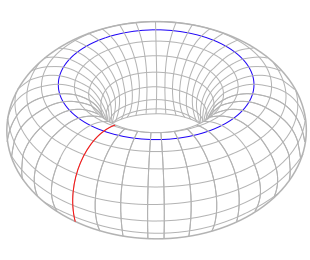
\includegraphics[width=.4\textwidth]{homology}
	 \caption{\small Base de ciclos de $\TT^2$.}
	 \label{fig:toro}
       \end{figure}

       Para calcular las variables de acción-ángulo existe una técnica estándar, expuesta en todas las referencias clásicas \cite{arnold,goldstein,landau}. En primer lugar, si $M_a$ es un toro de Liouville entonces su primer grupo de homología es
       \begin{equation*}
	 H_1(M_a)=H_1(\mathbb{T} ^n)=\mathbb{Z} ^n
       \end{equation*}
       y podemos tomar una base de ciclos $\left\{ \gamma_1,\dots,\gamma_n \right\}$ (ver figura \ref{fig:toro}). Definimos entonces las variables de acción
       \begin{equation}
	 J_i=\oint_{\gamma_i} \vect{p} d \vect{q}
       \end{equation}
       y construimos una transformación canónica $(\vect{q},\vect{p})\mapsto (\vect{J},\vect{w})$ generada por la función
       \begin{equation}
	 S(\vect{q},\vect{J})=\int_{\vect{q}_0}^{\vect{q}}\vect{p}(\vect{J},\vect{q}) \dd \vect{q} ,	
       \end{equation}
       donde esta integral está realizada a lo largo de una curva cualquiera (se puede demostrar que la elección de ésta no influye) que una $\vect{q}_0$ y $\vect{q}$ en $M_a$. Obtenemos ahora las variables de ángulo en la forma
       \begin{equation}
	 w_i=\frac{\partial S}{\partial J_i}. 
       \end{equation}

  \section{Sistemas superintegrables, trayectorias cerradas y simetrías ocultas}
  Podemos considerar ahora qué sucedería si un sistema integrable con $n$ grados de libertad tuviera cantidades conservadas adicionales, hasta otras $n-1$ para que puedan existir trayectorias, funcionalmente independientes de las anteriores, aunque ya no podrían estar en involución con todas. Esto motiva entonces la noción de \emph{superintegrabilidad} o \emph{integrabilidad no abeliana}.
  \begin{defn}
    Un sistema hamiltoniano con $n$ grados de libertad se dice \emph{superintegrable} si admite $n+k$ integrales primeras funcionalmente independientes para cierto $k=1,\dots,n-1$. En el caso en que $k=n-1$ el sistema se dice \emph{maximalmente superintegrable}.
  \end{defn}

  Las dos primeras partes del teorema \ref{arnoldliouville} se pueden generalizar al caso superintegrable, es lo que se conoce como el \emph{teorema de Mishchenko-Fomenko} \cite{mishchenko}. Destaca especialmente el caso maximalmente superintegrable, para el cual el resultado nos dice que las órbitas serán curvas cerradas con movimiento periódico.

  Vamos a aplicar estas ideas al caso del potencial central, para ver en qué casos el sistema será superintegrable. Como ya hemos visto, en el movimiento en un potencial central, el momento angular $\vect{L}=\vect{q}\times \vect{p}$ se conserva. Puesto que $\vect{L}$ es perpendicular a $\vect{q}$ y a $\vect{p}$, la conservación de $\vect{L}$ significa que, durante todo el movimiento, la posición y el momento de la partícula permanecen en un mismo plano, perpendicular a $\vect{L}$. La invariancia bajo rotaciones nos permite escoger la dirección $\vect{e}_z$ paralela al momento angular $\vect{L}$ y estudiar el sistema «reducido» en el plano perpendicular, que ahora será el plano $XY$. Llamando ahora $r=x^2+y^2$, el hamiltoniano en este «sistema reducido» será
  \begin{equation}
    H(x,y,p_x,p_y)= \tfrac{1}{2m}(p_x^2+p_y^2)+V(r).
  \end{equation}
  Cambiando a coordenadas polares $\vect{q}=(x,y)=r\vect{e}_{r}$, con $\vect{e}_r=(\cos \phi, \sin \phi)$, $p_r=m\dot r$, $p_{\phi}=mr^2\dot \phi$, tenemos
  \begin{equation}
    H(r,\phi,p_r,p_{\phi})=\frac{p_r^2}{2m}+\frac{p_{\phi}^2}{2mr^2}+V(r). 
  \end{equation}
  Nótese ahora que, si $\vect{p}=m\dot{\vect{q}}=m\dot r \vect{e}_r + mr \dot \phi \vect{e}_{\phi}$, con $\vect{e}_{\phi}=(-\sin \phi,\cos \phi)$, entonces $\vect{L}=\vect{q}\times \vect{p}=mr^2\dot \phi \vect{e}_z$, luego $L=|\vect{L}|=p_{\phi}$. Por tanto, el hamiltoniano queda en la forma
  \begin{equation}
    H(r,\phi,p_r,p_{\phi})=\frac{p_r^2}{2m}+\frac{L^2}{2mr^2}+V(r). 
  \end{equation}
  Al haber restringido el sistema a un plano y quedarnos con sólo dos grados de libertad, la integrabilidad sigue garantizada por la conservación del momento angular, mientras que la existencia de una cantidad conservada adicional independiente del momento angular nos daría la superintegrabilidad.

  Las trayectorias de energía $E$ y momento angular $L$ verificarán entonces las ecuaciones
  \begin{equation}
    \begin{cases}
    E=\tfrac{1}{2}m\dot r^2+\frac{L^2}{2mr^2}+V(r) \\
    L=mr^2\dot \phi.
  \end{cases}
  \end{equation}
  De modo que
  \begin{equation}
      \dot r=\sqrt{\frac{2}{m}[E-V(r)]-\frac{L^2}{2mr^2}} 
  \end{equation}
  y 
  \begin{equation}
    t=\int \frac{dr}{\sqrt{\frac{2}{m}[E-V(r)]-\frac{L^2}{2mr^2}}}.
  \end{equation}
  Por tanto, el ángulo $\phi$ puede ser integrado por cuadraturas en la forma
  \begin{equation}
    \phi=\int\frac{Ldr}{r^2\sqrt{2m[E-V(r)]-L^2/r^2}}. 
    \label{eq:intphi}
  \end{equation}

Observemos que podemos considerar la partícula sujeta a un «potencial efectivo»
\begin{equation}
  U=\frac{L^2}{2mr^2}+V(r),
\end{equation}
donde el término $\frac{L^2}{2mr^2}$ constituye una «energía centrífuga». En los valores de $r$ para los cuales $U$ es constante la velocidad radial $\dot r$ se anula y nos indica los \emph{puntos de retorno} de la trayectoria. En el caso en que el movimiento sea acotado, $r$ varía entre dos límites $r_{\text{min}}$ y $r_{\text{máx}}$ y la trayectoria está contenida enteramente en el interior de una corona circular limitada por las circunferencias de radios $r_{\text{min}}$ y $r_{\text{máx}}$. Sin embargo, esto no implica que la trayectoria sea una curva cerrada. En efecto, si, de acuerdo con \eqref{eq:intphi}, calculamos el ángulo que gira el vector posición en lo que la partícula se mueve entre $r_{\text{min}}$ y $r_{\text{máx}}$ obtenemos
\begin{equation}
  \Delta \phi = 2\int_{r_{\text{min}}}^{r_{\text{máx}}} \frac{Ldr}{r^2\sqrt{2m[E-V(r)]-L^2/r^2}}.
\end{equation}
La condición que ha de cumplirse para que la trayectoria en cierto momento se cierre es precisamente que este ángulo sea un múltiplo racional de $2\pi$, es decir, que $\Delta \phi = \frac{2\pi m}{n}$, para ciertos enteros $m$ y $n$. En un caso general esta condición no se cumple y la trayectoria va llenando densamente toda la corona en la que se encuentra contenida (ver figura \ref{fig:bertrand}).

\begin{figure}[h!]
  \centering
  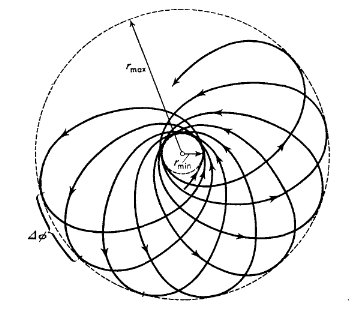
\includegraphics[width=.4\textwidth]{bertrand}
  \caption{\small Avance del ángulo de $r_{\text{máx}}$ (Fuente: \cite{landau}).}
  \label{fig:bertrand}
\end{figure}


J. Bertrand probó en 1883 \cite{bertrand} que precisamente los únicos potenciales centrales en los cuales todos los movimientos acotados se dan en trayectorias cerradas son aquellos en los que $V(r)$ es proporcional a $1/r$ (potencial de Kepler) o a $r^2$ (oscilador armónico isótropo). Por tanto, en el resto de casos el sistema no es superintegrable. Cabe preguntarse entonces si tanto el potencial de Kepler como el oscilador armónico isótropo tendrán alguna integral primera adicional que nos garantice la superintegrabilidad, tal vez dada por una «simetría oculta» del sistema, es decir, por una simetría que no era aparente a primera vista.

La respuesta es afirmativa en los dos casos. En el potencial de Kepler $V(r)=k/r$ existe una cantidad conservada adicional que es el \emph{vector de Laplace-Runge-Lenz} \cite{goldstein}, definido por
\begin{equation}
  \vect{A}=\vect{p}\times \vect{L}-mk\frac{\vect{q}}{r}. 
\end{equation}
En el caso del oscilador armónico isótropo $V(r)=kr^2$ existe un tensor simétrico conservado, el \emph{tensor de Fradkin} \cite{fradkin}, dado por
\begin{equation}
  A_{ij}=\tfrac{1}{2m}(p_ip_j+kq_iq_j), 
\end{equation}
con $i,j=1,2$. La traza del tensor es precisamente la energía $\tfrac{1}{2m}(\vect{p}^2+kr^2)$ y la componente de fuera de la diagonal $F=A_{12}=\tfrac{1}{2m}(p_1p_2+kq_1q_2)$ es precisamente la cantidad conservada adicional, indepentiende de la energía y del momento angular. 

Si se regresa al espacio tridimensional y se consideran ahí las cantidades conservadas adicionales ahora obtenidas, se pueden calcular las relaciones entre las diferentes integrales primeras del sistema con el corchete de Poisson y ver qué subalgebra de Lie del álgebra total de las variables dinámicas del sistema generan, desvelando así el verdadero rostro de estas «simetrías ocultas». Se puede probar que para el caso del potencial de Kepler esta álgebra es $\mathfrak{so}(4)$ mientras que para el caso del oscilador armónico isótropo es $\mathfrak{su}(3)$.

Para terminar la sección, cabe comentar que la superintegrabilidad de un sistema clásico también tiene sus consecuencias en Mecánica Cuántica. Por ejemplo, en el caso del átomo de hidrógeno (que se puede considerar el análogo cuántico del problema de Kepler, de modo que conserva las mismas simetrías) la existencia de la cantidad conservada adicional, el vector de Laplace-Runge-Lenz, es la causante de la degeneración «accidental» de sus niveles de energía. Por degeneración accidental de los niveles del átomo de hidrógeno nos referimos al hecho de que sus niveles de energía dependan tan solo del primer número cuántico, $n$, y no del número cuántico $l$.

\section{El oscilador armónico anisótropo}
En esta sección estudiamos la superintegrabilidad de otro sistema clásico, el oscilador armónico anisótropo. Para encontrar las integrales primeras adicionales nos ayudaremos de unas coordenadas complejas adicionales, que nos permitirán encontrar un tensor conservado. Este procedimiento se debe a J.M. Jauch y E. L. Hill \cite{jauchhill} y sus ideas principales nos serán útiles más adelante para tratar otros problemas.

El oscilador armónico anisótropo con $n$ grados de libertad está definido sobre el espacio de fases $\RR^{2n}=\left\{ \vect{q},\vect{p} \right\}$ y su hamiltoniano viene dado por
\begin{equation}
  H(\vect{q},\vect{p})=\frac{1}{2}\sum_{i=1}^n \left(p_i^2 + \omega_i^2q_i^2\right)=\sum_{i=1}^n H_i(q_i,p_i),
  \label{eq:anisotropo}
\end{equation}
con $H_i(q_i,p_i)=\frac{1}{2}(p_i^2+\omega_i^2q_i^2)$. Para probar la integrabilidad del sistema basta tomar las funciones $H_i$, ya que
\begin{equation*}
  \left\{ H_i,H_j \right\}=\parcial{H_i}{p_k}\parcial{H_j}{q_k}-\parcial{H_j}{p_k}\parcial{H_i}{q_k}=0.
\end{equation*}

Los conjuntos de nivel de las funciones $F_j(\vect{q},\vect{p})=a_j$ serán toros de Liouville dados por las ecuaciones
\begin{align*}[left=\empheqlbrace]
    p_1^2+\omega_1^2q_1^2&= 2a_1\\
    p_1^2+\omega_2^2q_1^2&= 2a_2\\
    &\vdotswithin{=} \\
    p_n^2+\omega_n^2q_n^2&= 2a_n.
\end{align*}
Es posible demostrar que las trayectorias del flujo hamiltoniano en estos toros son cerradas si y sólo si las frecuencias $\omega_i$ son de la forma $\omega_i=n_i \omega$, para cierta $\omega$ y para ciertos números enteros $n_i$, de modo que el hamiltoniano \eqref{eq:anisotropo} toma la forma
\begin{equation}
  H(\vect{q},\vect{p})=\frac{1}{2}\sum_{i=1}^n \left(p_i^2 + n_i^2\omega^2q_i^2\right).
\end{equation}
Veamos entonces que precisamente en estos casos el oscilador armónico anisótropo es superintegrable.

Para encontrar las integrales primeras adicionales vamos a servirnos de un espacio de fases complejo auxiliar $\CC^n$, con coordenadas $z_i, \bar{z}_i$. Concretamente, definimos
\begin{equation}
  z_j=p_j-in_j\omega q_j,\ \ \  \bar{z}_j=p_j+in_j\omega q_j.  
\end{equation}
Tenemos entonces que $H_i=\frac{1}{2}z_i\bar{z}_i$ y el hamiltoniano es de la forma
\begin{equation}
  H=\frac{1}{2}\sum_{i=1}^n z_i\bar{z}_i. 
\end{equation}
Ahora, se comprueba fácilmente que las cantidades
\begin{equation}
  c_{ij}=z_i^{n_j}\bar{z}_j^{n_i} 
\end{equation}
son integrales primeras del sistema. En el caso en que $n_i=n_j$, entre estas cantidades tenemos los momentos angulares
\begin{equation}
  L_{ij}=q_ip_j-q_jp_i 
\end{equation}
y un tensor similar al de Fradkin
\begin{equation}
  A_{ij}=p_ip_j+n_in_j\omega^2 q_iq_j. 
\end{equation}

\section{El hamiltoniano de TTW}
Principalmente por consideraciones al cuantizar, dentro de los sistemas integrables y superintegrables son de especial interés aquellos en los que sus integrales primeras son polinomiales en los momentos. Así, estos sistemas se llamarán \emph{polinomialmente integrables} (respectivamente, \emph{polinomialmente superintegrables}) y llamaremos \emph{orden} de sus integrales primeras al grado que estas tengan como polinomios en los momentos. Para más información al respecto, consultar \cite{miller}.

Los sistemas superintegrables de segundo orden han sido bastante estudiados y poseen una teoría de clasificación. También han sido tratados varias clases de sistemas de tercer orden. Sin embargo, para sistemas generales de tercer orden y de órdenes superiores se conoce mucho menos. En particular hasta hace unos pocos años había pocos ejemplos y las teorías de estructura y clasificación eran prácticamente inexistentes. 

La situación cambió drásticamente en 2009 con el trabajo de F. Tremblay, A. V. Turbiner y P. Winternitz \cite{ttw1}, donde los autores presentaron una familia de potenciales en el plano, parametrizados por una constante $k$, y conjeturaron que estos sistemas eran superintegrables para todo $k\in \QQ$, con órdenes tan grandes como se quisieran. Unos meses más tarde, en otro trabajo \cite{ttw2} los mismos autores calcularon las trayectorias acotadas de esta familia de sistemas y mostraron que eran curvas cerradas para todos los casos con $k \in \QQ$, dando así evidencia a favor de su conjetura. Posteriormente se ha verificado por varios métodos que, efectivamente, sus conjeturas eran correctas.

Concretamente, el hamiltoniano de Tremblay, Turbiner y Winternitz (que a partir de ahora abreviaremos como \emph{hamiltoniano de TTW}) en coordenadas polares tiene la forma 
\begin{equation}
  H_k(r,\phi,p_r,p_{\phi})=\frac{1}{2}\left( p_r^2+\frac{p^2_{\phi}}{r^2} +\omega^2 r^2 \right) + V_k(r,\phi),
\end{equation}
con
\begin{equation}
  V_k(r,\phi)=\frac{\alpha k^2}{2r^2\cos^2 k\phi}+\frac{\beta k^2}{2r^2\sin^2 k\phi}.
  \label{eq:TTW}
\end{equation}
La integrabilidad viene garantizada por la integral primera
\begin{equation}
  X_k=p_{\phi}^2+\frac{\alpha k^2}{\cos^2 k\phi}+\frac{\beta k^2}{\sin^2 k\phi}.
  \label{eq:integralprimeraTTW}
\end{equation}
La existencia de una integral primera adicional $Y_{k}$ para $k\in \QQ$ que diera la superintegrabilidad polinomial del sistema fue conjeturada por Tremblay, Turbiner y Winternitz en \cite{ttw1} y posteriormente demostrada.

\section{Superintegrabilidad del sistema de TTW}
En esta sección vamos a demostrar la superintegrabilidad del sistema de TTW con $k\in \QQ$ siguiendo el método de C. Gonera \cite{gonera}. Para ello, lo primero que vamos a hacer es obtener las variables de acción-ángulo del sistema. Teniendo en cuenta que las integrales primeras que dan la integrabilidad son el hamiltoniano $\eqref{eq:TTW}$ y la función $X_k$ dada por $\eqref{eq:integralprimeraTTW}$, un toro de Liouville con $H=E$ y $X_k=A$ vendrá dado por las ecuaciones
\begin{equation}
  \begin{cases}
    p_r^2+\frac{p_{\phi}^2}{r^2}+\omega^2r^2 + \frac{k}{r^2}\left( \frac{\alpha}{\cos^2k\phi} +\frac{\beta}{\sin^2k\phi}\right) = 2E \\
    p_{\phi}^2+k^2\left( \frac{\alpha}{\cos^2k\phi} +\frac{\beta}{\sin^2k\phi}\right)=A.
  \end{cases}
\end{equation}

Para que los cálculos sean más sencillos vamos a realizar un cambio de coordenadas 
\begin{equation}
 \theta=k\phi. 
\end{equation}
Si consideramos ahora el lagrangiano asociado al sistema TTW en coordenadas polares
\begin{equation}
  \mathcal{L} _k(r,\phi,\dot{r},\dot{\phi})=\frac{1}{2}\left(\dot{r}^2+r^2\dot{\phi}^2-\omega r^2\right)-V_k(r,\phi), 
\end{equation}
podemos escribir
\begin{equation}
  \mathcal{L} _k(r,\theta,\dot{r},\dot{\theta})=\frac{1}{2}\left(\dot{r}^2+\frac{r^2}{k^2}\dot{\theta}^2-\omega r^2\right)-V_k(r,\theta), 
\end{equation}
con
\begin{equation}
  V_k(r,\theta)=\frac{\alpha k^2}{2r^2\cos^2 \theta}+\frac{\beta k^2}{2r^2\sin^2 \theta}.
\end{equation}
Ahora, el momento canónico conjugado de $\theta$ sera
\begin{equation}
  p_\theta=\frac{\partial \mathcal{L} }{\partial \dot{\theta}}=\frac{r^2}{k^2}\dot{\theta}. 
\end{equation}
Teniendo en cuenta ahora que $\dot{\theta}=k\dot{\phi}$ y que $p_{\phi}=r^2\dot{\phi}$, tenemos
\begin{equation}
  p_{\phi}=kp_\theta. 
\end{equation}
De modo que en las nuevas coordenadas el hamiltoniano es
\begin{equation}
  H_k(r,\theta,p_r,p_{\theta})=\frac{1}{2}\left( p_r^2+\frac{k^2}{r^2}p^2_{\theta} +\omega^2 r^2 \right) + V_k(r,\theta),
\end{equation}
y la integral primera $X_k$ se escribe
\begin{equation}
  X_k=k^2p_{\theta}^2+\frac{\alpha k^2}{\cos^2 \theta}+\frac{\beta k^2}{\sin^2 \theta}.
\end{equation}
Por tanto, podemos redefinir entonces la constante $A=\frac{A}{k^2}$ y el toro de Liouville queda
\begin{equation}
  \begin{cases}
    p_r^2+\frac{k^2}{r^2}p_{\theta}^2+\omega^2r^2 + \frac{k^2}{r^2}\left( \frac{\alpha}{\cos^2\theta} +\frac{\beta}{\sin^2\theta}\right) = 2E \\
    p_{\theta}^2+ \frac{\alpha}{\cos^2\theta} +\frac{\beta}{\sin^2\theta}=A.
  \end{cases}
  \label{eq:toro}
\end{equation}

Para obtener ahora las variables de acción tomamos como base de ciclos del toro de Liouville los cortes de éste con los planos $(r,p_r)$ y $(\theta,p_{\theta})$, de modo que podemos definir
\begin{align}
    J_r=\frac{1}{2\pi}\oint p_r dr, \\
    J_\theta=\frac{1}{2\pi}\oint p_{\theta}d\theta,
\end{align}
donde las integrales se realizan precisamente en estos ciclos que hemos tomado (ver figura \ref{fig:ciclos}). Los cortes de estos ciclos con los ejes $r$ y $\theta$, respectivamente, serán precisamente las raíces de las expresiones que se obtienen al despejar en las ecuaciones \eqref{eq:toro} 
\begin{align}
    p_r=\sqrt{2E-\omega^2r^2-\frac{k^2}{r^2}A}, \\
    p_{\theta}=\sqrt{A-\frac{\alpha}{\cos^2\theta} -\frac{\beta}{\sin^2\theta}}.
\end{align}
Podemos calcular entonces las integrales
\begin{align}
  J_r=\frac{1}{2\pi}\oint \sqrt{2E-\omega^2r^2-\frac{k^2}{r^2}A} dr=\frac{E}{2\omega}-\frac{k\sqrt{A}}{2}, \label{eq:intaccion1} \\ 
  J_\theta=\frac{1}{2\pi}\oint \sqrt{A-\frac{\alpha}{\cos^2\theta} -\frac{\beta}{\sin^2\theta}}d\theta=\frac{\sqrt{A}}{2}-\frac{\sqrt{\alpha}+\sqrt{\beta}}{2}. 
\label{eq:intaccion2}
\end{align}
Como $\frac{\sqrt{\alpha}+\sqrt{\beta}}{2}$ es un término que sólo depende de $\alpha$ y $\beta$ podemos redefinir trivialmente 
\begin{equation}
  J_{\theta}=\frac{\sqrt{A}}{2}. 
\end{equation}
El cálculo de la integral \eqref{eq:intaccion1} puede hacerse con técnicas de variable compleja, como aparece detallado en el Apéndice \ref{apendice}, mientras que la integral \eqref{eq:intaccion2} está calculada usando técnicas elementales en \cite{lechtenfeld}.

\begin{figure}[h]
  \centering
  \includegraphics{ciclos}
  \caption{\small Ciclos del toro de Liouville y variables de acción.}
  \label{fig:ciclos}
\end{figure}

Una vez obtenidas las variables de acción, despejamos para obtener el hamiltoniano
\begin{equation}
  H(J_r,J_\theta,w_r,w_\theta)=2\omega(J_r+kJ_\theta),
\end{equation}
donde $w_r$ y $w_\theta$ son las variables angulares que, por las ecuaciones de Hamilton, verifican
\begin{equation}
  \begin{cases}
    \nu_r=\dot{w}_r=\frac{\partial H}{\partial J_r}=2\omega, \\ 
    \nu_{\theta}=\dot{w}_{\theta}=\frac{\partial H}{\partial J_\theta}=2\omega k.
  \end{cases}
\end{equation}
Ahora, si $k$ es irracional, entonces las frecuencias $\nu_r$ y $\nu_\theta$ no son conmesurables y las trayectorias son densas en el toro de Liouville \cite{arnold}, de forma que en ese caso el sistema no puede ser superintegrable. En el caso en que $k=\frac{m}{n}$, con $m,n \in \NN$ entonces claramente
\begin{equation*}
  m\dot{w}_r-n\dot{w}_\theta=0,
\end{equation*}
luego 
\begin{equation}
  mw_r-nw_\theta
\end{equation}
es una constante del movimiento que además por construcción es independiente de $J_r$ y de $J_\theta$, luego de $H$ y $X_k$. En conclusión, tenemos que el sistema de TTW es superintegrable si y sólo si $k\in \QQ$.

Una sutileza a tener en cuenta es que $2mw_r-nw_\theta$ es una función multivalorada en el toro de Liouville, pero este problema se soluciona fácilmente si, siguiendo la idea de \cite{landau}, consideramos una función trigonométrica de esta magnitud, por conveniencia
\begin{equation}
  e^{i(mw_r-nw_{\theta})}=(e^{iw_r})^{m}(e^{-iw_{\theta}})^n.
\end{equation}
Si nos resulta de interés, se pueden calcular las variables angulares explícitamente siguiendo el método explicado en la sección 2 y de ahí obtener el valor de la integral primera adicional. Aunque aquí no lo detallemos (el cálculo completo puede leerse en \cite{gonera}), la cantidad que se obtiene es (en las coordenadas polares originales y tras algunas simplificaciones)
\begin{equation}
  Y_{k}=\left[ \frac{2\sqrt{A}p_r}{r}+i\left( E-\frac{2A}{r^2} \right) \right]^m\left[\sqrt{A}p_{\phi}\sin 2k\phi + i\left[ (\beta-\alpha)k^2+A\cos2k\phi \right] \right]^n.
\end{equation}
Una comprobación directa muestra que $Y_{k}$ es una integral primera independiente de $H$ y de $X_k$ y que, por tanto, el sistema de TTW es superintegrable cuando $k$ es racional. Nótese además que la integral $Y_k$ es polinomial en los momentos $p_r$ y $p_\theta$.

\section{El hamiltoniano de TTW en coordenadas cartesianas}
Para continuar con el estudio del Hamiltoniano de TTW, en esta sección vamos a ver cómo se expresa en coordenadas cartesianas y vamos a representar el potencial en los casos más sencillos.

En coordenadas cartesianas, el hamiltoniano de TTW toma la forma
\begin{equation}
  H_k(x,y,p_x,p_y)=\frac{1}{2}[p_x^2+p_y^2+\omega^2(x^2+y^2)]+V_k(x,y),
\end{equation}
a falta de hallar el aspecto del potencial $V_k$ en coordenadas cartesianas.
Teniendo en cuenta que $(x,y)=r\vect{e}_r$, en coordenadas cartesianas el potencial queda
\begin{align}
  V_k(x,y)=\frac{\alpha k^2}{2r^2\cos^2(k\arctan \tfrac{y}{x})} +\frac{\beta k^2}{2r^2\sin^2(k\arctan \tfrac{y}{x})}
\end{align}
o, equivalentemente,
\begin{align}
  V_k(x,y)=\frac{k^2}{2(x^2+y^2)}\left( \alpha\left[ 1+\tan^2\left( k\arctan\frac{y}{x} \right) \right] \right. \left. +\beta\left[ 1+\cot^2\left( k\arctan\frac{y}{x} \right) \right]\right).
\end{align}
Esta expresión solo es sencilla para algunos valores de $k$, por ejemplo, para $k=1$,
\begin{equation}
  V_1=\frac{1}{2}\left( \frac{\alpha}{x^2}+\frac{\beta}{y^2} \right).
\end{equation}
Para valores enteros pequeños de $k$ podemos hacer algunas simplificaciones y obtenemos
\begin{equation}
  V_2=\frac{1}{2}(x^2+y^2)\left( \frac{4\alpha}{(x^2-y^2)^2}+\frac{\beta}{x^2y^2} \right)
\end{equation}
y
\begin{equation}
  V_3=\frac{9}{2}(x^2+y^2)^2\left( \frac{\alpha}{(x^3-3xy^2)^2}+\frac{\beta}{(-3x^2y+y^3)^2} \right).
\end{equation}
Destaca también el caso con $k=\tfrac{1}{2}$,
\begin{equation}
  V_{1/2}=\frac{1}{2y^2}\left[ \alpha\left( 1-\frac{x}{\sqrt{x^2+y^2}} \right)+ \beta\left( 1+\frac{x}{\sqrt{x^2+y^2}} \right) \right].
\end{equation}

\section{El hamiltoniano de TTW en coordenadas complejas}
Inspirados por el cambio a coordenadas complejas que hemos hecho al tratar el oscilador armónico anisótropo, vamos a tratar de introducir unas coordenadas complejas al caso del hamiltoniano TTW, para ver si lo podemos dejar en una forma que nos dé más información sobre su comportamiento. En este caso, sin embargo, el cambio propuesto es ligeramente distinto, ya que no queremos combinar las coordenadas con los momentos sino que queremos obtener unas nuevas coordenadas generalizadas complejas y ver qué aspecto tendrán sus momentos canónicos conjugados. Concretamente, queremos hacer un cambio de esta forma
\begin{equation}
  z=x+iy.
\end{equation}
Esta clase de tratamientos de las coordenadas generalizadas son realizados comúnmente en física en diversas situaciones, sin embargo, cabe detenerse por un momento para entender qué es lo que está sucediendo geométricamente.

Sea $M$ una variedad diferenciable. Una \emph{estructura cuasicompleja} en $M$ es un endomorfismo
\begin{align*}
  J :TM&\longrightarrow TM
  \end{align*}
  tal que $J^2=-\mathrm{id}$. Nótese que por tanto $M$ ha de tener dimensión par. Podemos considerar entonces el \emph{fibrado tangente complexificado}
  \begin{equation*}
    T_{\CC}M=TM\otimes \CC.
  \end{equation*}
Ahora, si consideramos la aplicación bilineal
\begin{align*}
  \tilde{J} :TM \times \CC&\longrightarrow TM\otimes \CC\\ 
    (\xi,z) &\longmapsto J(\xi)\otimes \CC, 
  \end{align*}
  entonces, por la propiedad universal del producto tensorial existe una única aplicación lineal $I:T_{\CC}M \rightarrow T_{\CC}M$ tal que el siguiente diagrama conmuta
  \begin{center}
    \begin{tikzcd}
      TM \times \CC      \arrow{rr}{\otimes}\arrow{rrdd}[anchor=north,rotate=-30]{\tilde{J}} && T_{\CC}M = TM \otimes \CC \arrow{dd}[anchor=west]{I} \\ 
       && \\
       &&T_{\CC}M.
     \end{tikzcd}
   \end{center}
   La aplicación $I$ es entonces un endomorfismo de $T_{\CC}M$ con autovalores $\pm i$ y podemos descomponer
   \begin{equation*}
     T_{\CC}M=\ker(I-i)\oplus \ker(I+i).
   \end{equation*}

   En el caso particular en que $M$ se una variedad de dimensión $2$ con coordenadas $(x,y)$, podemos considerar entonces la «coordenada compleja» 
   \begin{equation*}
     z=x+iy.
   \end{equation*}
   Ahora, en el fibrado tangente $TM$ podemos considerar la base holónoma $\left\{ \partial_x, \partial_y \right\}$ y la estructura cuasicompleja dada por
   \begin{align*}
     I :TM&\longrightarrow TM\\ 
       \partial_x &\longmapsto \partial_y \\
       \partial_y &\longmapsto -\partial_x .
     \end{align*}
     Consideremos entonces el fibrado tangente complexificado $T_{\CC}M$ y los vectores
     \begin{equation}
       \begin{cases}
	 \partial_z=\tfrac{1}{2}(\partial_x-i\partial_y) \\
	 \partial_{\bar{z}}=\tfrac{1}{2}(\partial_x+i\partial_y) .
       \end{cases}
     \end{equation}
     Es inmediato comprobar que 
	 $\partial_z\in \ker(I-i)$ y que
	 $\partial_{\bar{z}} \in \ker(I+i)$,
	 de modo que $\left\{ \partial_z, \partial_{\bar{z}} \right\}$ es una base de $T_{\CC}M$. Si tenemos un vector $v \in TM$ que en la base holónoma original se escribe
     \begin{equation}
       v = \dot{x} \partial_x + \dot{y} \partial_y,
     \end{equation}
     entonces, si pensamos en $v$ como vector de $T_{\CC}M$, podemos escribirlo en la base $\left\{ \partial_z, \partial_{\bar{z}} \right\}$ en la forma
     \begin{equation}
       v= \dot{z} \partial_z + \dot{\bar{z}} \partial_{\bar{z}},
     \end{equation}
     con $\dot{z}=\dot{x} + i \dot{y}$. De modo que un lagrangiano $\mathcal{L}:TM\rightarrow \RR$, que localmente puede expresarse en las coordenadas originales
     \begin{equation}
       \mathcal{L}(v)=\mathcal{L}(x,y,\dot{x},\dot{y}),
     \end{equation}
     puede extenderse a $T_{\CC}M$ en las nuevas coordenadas complejas en la forma
     \begin{equation}
       \mathcal{L} (v)=\mathcal{L}(z,\bar{z},\dot{z},\dot{\bar{z}}).
     \end{equation}

     Volviendo al caso que nos incumbe, $M=\RR^2$ y podemos considerar el lagrangiano del sistema TTW
     \begin{equation}
       \mathcal{L}_k(x,y,\dot{x},\dot{y})=\tfrac{1}{2}[\dot{x}^2+\dot{y}^2-\omega^2(x^2+y^2)]-V_k(x,y).
     \end{equation}
     Tomamos ahora el potencial $V_k$ en coordenadas polares
\begin{equation}
  V_k(r,\phi)=\frac{\alpha k^2}{2r^2\cos^2 k\phi}+\frac{\beta k^2}{2r^2\sin^2 k\phi}
\end{equation}
y lo cambiamos a las nuevas coordenadas
\begin{equation}
  \begin{cases}
    z=x+iy \\
    \bar{z}=x-iy,
  \end{cases}
\end{equation}
teniendo en cuenta que $z=r e^{i\phi}$ y la fórmula de Moivre
\begin{equation*}
  z^k=r^k(\cos k\phi+i\sin k\phi),
\end{equation*}
de donde se tiene
\begin{equation*}
  \cos k\phi = \frac{z^k+\zz^k}{2|z|^k} \ \  \sin k\phi = \frac{z^k-\zz^k}{2i|z|^k}. 
\end{equation*}
Obtenemos entonces el potencial
\begin{equation}
V_k(z,\zz)=2k^2z^{k-1}\zz^{k-1}\left[\frac{\alpha  }{(z^k+\zz^k)^2}-\frac{\beta  }{(z^k-\zz^k)^2}\right].
\end{equation}
De modo que el lagrangiano del sistema TTW se expresa en las coordenadas complejas en la forma
\begin{equation}
  \mathcal{L}_k(z,\zz,\dot{z},\dot{\zz})=\tfrac{1}{2}(\dot{z}\dot{\zz}-\omega^2 z \zz) - V_k(z,\zz).
\end{equation}
Ahora, teniendo en cuenta que, en este caso,
\begin{equation}
  \begin{cases}
    p_x=\dot{x}\\
    p_y=\dot{y},
  \end{cases}
\end{equation}
tenemos los nuevos momentos canónicos conjugados
\begin{equation}
  \begin{cases}
    p_z=\frac{\partial \mathcal{L}_k }{\partial \dot{z}}=\tfrac{1}{2} \dot{\zz}=\tfrac{1}{2}(\dot{x}-i\dot{y})=\tfrac{1}{2}(p_x-ip_y),\\
    p_{\zz}=\frac{\partial \mathcal{L}_k }{\partial \dot{\zz}}=\tfrac{1}{2} \dot{z}=\tfrac{1}{2}(\dot{x}+i\dot{y})=\tfrac{1}{2}(p_x+ip_y).
  \end{cases}
\end{equation}
Vemos entonces que el hamiltoniano de TTW se escribe en las coordenadas complejas en la forma
\begin{equation}
  H_k(z,\zz,p_z,p_{\zz})=\tfrac{1}{2}(p_zp_{\zz}+\omega^2 z \zz) + V_k(z,\zz).
\end{equation}
Nótese también que podemos seguir pensando en las coordenadas $(z,\zz,p_z,p_{\zz})$ como coordenadas de Darboux, en efecto, se comprueba fácilmente que
\begin{equation}
  \dd p_z \wedge \dd z + \dd p_{\zz} \wedge \dd \zz=\dd p_x \wedge \dd x + \dd p_y \wedge \dd y.
\end{equation}
Finalmente, observamos que si $k=1$ recuperamos el oscilador armónico con términos centrífugos (barreras de Rosochatius)
\begin{equation}
  V_1=\frac{2\alpha}{(z+\zz)^2}-\frac{2\beta}{(z-\zz)^2},
\end{equation}
y, cuando $k$ sea entero, el potencial será una función racional
\begin{align}
  V_k=2k^2(x^2+y^2)^{k-1}\left[ \frac{\alpha}{\left( (x+iy)^k+(x-iy)^k \right)^2}-\frac{\beta}{\left( (x+iy)^k-(x-iy)^k \right)^2} \right].
\end{align}

\section{El hamiltoniano de TTW en unas nuevas coordenadas}
Vamos a estudiar ahora el sistema de TTW en unas nuevas coordenadas reales, definidas de la siguiente manera
\begin{equation}
  \begin{cases}
    u=\tfrac{1}{2}(z^k+\zz^k)=r^k\cos k\phi, \\
    v=\tfrac{1}{2i}(z^k-\zz^k)=r^k \sin k\phi.
  \end{cases}
\end{equation}
De modo que
\begin{equation}
  \begin{cases}
    \dot{u}=\tfrac{1}{2}(kz^{k-1}\dot{z}+k\zz^k\dot{\zz}),\\
    \dot{v}=\tfrac{1}{2i}(kz^{k-1}\dot{z}-k\zz^k\dot{\zz}).
  \end{cases}
\end{equation}
Notamos ahora que 
\begin{equation*}
  \begin{cases}
    \dot{u}+i\dot{v}=kz^{k-1}\dot{z},\\
    \dot{u}-i\dot{v}=k\zz^{k-1}\dot{\zz},
  \end{cases}
\end{equation*}
y que
\begin{equation*}
  u^2+v^2=(z\zz)^k.
\end{equation*}
Luego
\begin{equation*}
  z\zz=(u^2+v^2)^{\frac{1}{k}}
\end{equation*}
y
\begin{equation*}
    \dot{z}\dot{\zz}=\frac{(\dot{u}+i\dot{v})(\dot{u}-i\dot{v})}{k^2z^{k-1}\zz^{k-1}}=\frac{\dot{u}^2+\dot{v}^2}{k^2(u^2+v^2)^{\frac{k-1}{k}}}.
\end{equation*}
Obtenemos entonces que el lagrangiano en estas coordenadas se expresa
\begin{equation}
  \mathcal{L}_k(u,v,\dot{u},\dot{v})=\frac{1}{2}\left[ \frac{\dot{u}^2+\dot{v}^2}{k^2(u^2+v^2)^{\frac{k-1}{k}}} -\omega^2(u^2+v^2)^{\frac{1}{k}}\right]-V_k(u,v),
\end{equation}
con
\begin{equation}
  V_k(u,v)=k^2(u^2+v^2)^{\frac{k-1}{k}}\left[ \frac{\alpha}{2u^2}+\frac{\beta}{2v^2} \right].
\end{equation}

Podemos calcular ahora los momentos canónicos conjugados de estas coordenadas
\begin{equation}
  \begin{cases}
    p_u=\frac{\partial \mathcal{L} _k}{\partial \dot{u}}=\frac{\dot{u}}{k^2 (u^2+v^2)^{\frac{k-1}{k}}}, \\
    p_v=\frac{\partial \mathcal{L} _k}{\partial \dot{v}}=\frac{\dot{v}}{k^2 (u^2+v^2)^{\frac{k-1}{k}}},
  \end{cases}
\end{equation}
y el hamiltoniano
\begin{equation*}
  H_k=p_u \dot{u} + p_v \dot{v} - \mathcal{L}_k,
\end{equation*}
que finalmente tiene el siguiente aspecto
\begin{equation}
  H_k = k^2 (u^2+v^2)^{\frac{k-1}{k}}\left[ \frac{1}{2}(p_u^2+p_v^2)+ \frac{\omega^2}{2k^2}(u^2+v^2)^{\frac{2}{k}-1}+\frac{\alpha}{2u^2}+\frac{\beta}{2 v^2} \right]. 
\end{equation}
Lo interesante de ver el hamiltoniano en estas coordenadas es que, si se elimina el factor global $k^2(u^2+v^2)^{\frac{k-1}{k}}$, lo que obtenemos es un oscilador no lineal con términos centrífugos.

Esta manera de entender el hamiltoniano de TTW fue originalmente propuesta por M. A. Rodríguez (el director de este trabajo) y no publicada, aunque sí propuesta en un congreso. Muy recientemente el hamiltoniano de TTW ha sido estudiado en este aspecto por G. Gubbiotti y D. Latini en su trabajo \cite{gubbiottilatini}, donde sugieren un nuevo argumento a favor de su superintegrabilidad para $k$ racional empleando un método novedoso basado en la técnica de escalas múltiples.

\section{El hamiltoniano de TTW en espacios de curvatura constante}
En esta sección hacemos una breve exposición de las generalizaciones del hamiltoniano de TTW a la esfera $\mathbb{S} ^2$ y al plano hiperbólico $\mathbb{H} ^2.$ El estudio de sistemas de este tipo se remonta al trabajo de Higgs \cite{higgs}, donde trató con la generalización del oscilador armónico a la esfera. Siguiendo estas ideas, recientemente se han tratado generalizaciones de sistemas superintegrables conocidos a espacios de curvatura constante. Una exposición detallada de los métodos utilizados para estas generalizaciones puede encontrarse en \cite{ballesteros}. Concretamente, el estudio del hamiltoniano de TTW en estos espacios así como una demostración de su superintegrabilidad puede leerse en \cite{ranada}.

Para modelizar las geometrías esférica e hiperbólica seguimos el método clásico del programa de Erlangen, que consiste en tratar cada uno de estos espacios como un espacio homogéneo de un determinado grupo de isometrías actuando sobre $\mathbb{R}^3$. Así, en general el espacio a tratar vendrá modelizado por la superficie $S_\kappa \subset \mathbb{R} ^3$ de ecuación
\begin{equation}
 x_0^2+\kappa(x_1^2+x_2^2)=1. 
\end{equation}
Cuando $\kappa=1$ obtenemos una esfera, mientras que si $\kappa=-1$ obtenemos un hiperboloide de dos hojas y si $\kappa=0$ obtenemos dos planos. En los dos últimos casos nos interesa trabajar sólo en una de las dos hojas, por lo añadimos la restricción $x_0\geq 1$. Podemos dotar ahora a $S_\kappa$ de una métrica, restringiendo la métrica de $\mathbb{R} ^3$ y diviendo por la curvatura
\begin{equation}
  ds^2=\frac{1}{\kappa}(\dd x_0^2 +  \dd x_1^2 + \dd x_2^2)|_{S_\kappa}=\frac{\kappa (x_1\dd x_1+x_2 \dd x_2)^2}{1-\kappa(x_1^2+x_2^2)}+\dd x_1^2 + \dd x_2 ^2.
\end{equation}
De modo que el lagrangiano libre en $S_{\kappa}$ tomará la forma
\begin{equation}
  \mathcal{L} _\kappa=\frac{\kappa (x_1\dot{x}_1+x_2 \dot{x}_2)^2}{2[1-\kappa(x_1^2+x_2^2)]}+\frac{1}{2}(\dot{x}_1^2 + \dot{x}_2 ^2).
\end{equation}

Definimos ahora las \emph{coordenadas polares geodésicas} $(r,\phi)$, dadas por la relación
\begin{equation}
  \begin{cases}
    x_1=S_\kappa (r)\cos \phi\\
    x_2=S_\kappa (r)\sin \phi,
  \end{cases}
\end{equation}
donde $S_\kappa$ y $C_\kappa$ son las \emph{funciones trigonométricas generalizadas}, dadas por
\begin{equation}
  C_{\kappa}(x)=
  \begin{cases}
    \cos \sqrt{\kappa} x & \kappa >0, \\
    1 & \kappa =0, \\
    \cosh \sqrt{-\kappa} x & \kappa <0, 
  \end{cases}
\end{equation}
\begin{equation}
  S_{\kappa}(x)=
  \begin{cases}
    \frac{1}{\sqrt{\kappa}}\sin \sqrt{\kappa} x & \kappa >0, \\
    x & \kappa =0, \\
    \frac{1}{\sqrt{-\kappa}}\sinh \sqrt{-\kappa} x & \kappa <0. 
  \end{cases}
\end{equation}
Una comprobación directa muestra que el lagrangiano libre en estas coordenadas tiene la forma
\begin{equation}
  \mathcal{L} _\kappa = \frac{1}{2}(\dot{r}^2+S_{\kappa}^2 (r) \dot{\phi}^2).
\end{equation}
De modo que los momentos conjugados de las coordenadas geodésicas polares serán
\begin{align}
  p_r&=\dot{r} \\ 
  p_{\phi}&=S_{\kappa}^2(r) \dot{\phi}.
\end{align}
Luego el hamiltoniano libre toma la forma
\begin{equation}
  H_{\kappa}=\frac{1}{2}\left( p_r^2 + \frac{p^2_\phi}{S_{\kappa}^2(r)} \right) .
\end{equation}
Nótese que si $\kappa=0$ se obtienen las relaciones típicas de las coordenadas polares en el plano.
  
Siguiendo las ideas de Higgs \cite{higgs} de la generalización del oscilador armónico a la esfera, se puede definir el \emph{hamiltoniano de TTW generalizado} como
\begin{equation}
  H_{k,\kappa}=\frac{1}{2}\left( p_r^2 + \frac{p^2_\phi}{S_{\kappa}^2(r)}+ \omega^2 T_\kappa^2(r)\right) + V_{k,\kappa}(r,\phi)  ,
\end{equation}
donde $T_{\kappa}=\frac{S_\kappa}{C_\kappa}$ y
\begin{equation}
  V_{k,\kappa}(r,\phi)=\frac{k^2\alpha}{2S_\kappa^2(r)\cos^2k\phi} +\frac{k^2\beta}{2S_\kappa^2(r)\sin^2 k\phi}.
\end{equation}
Nótese que en el \emph{límite euclídeo}, cuando $\kappa\rightarrow 0$, se recupera el hamiltoniano de TTW en el plano \eqref{eq:TTW}. Varias consideraciones sobre este hamiltoniano y, en particular, una prueba de su superintegrabilidad para $k$ racional pueden leerse en \cite{ranada}.

\appendix
\section{Cálculo de la integral \eqref{eq:intaccion1}}\label{apendice}
En este apéndice vamos a detallar el cálculo de la integral \eqref{eq:intaccion1}. El método de integración que seguiremos es la técnica estándar presentada en \cite{goldstein}, donde se aplica al caso del problema de Kepler.

Para hallar la integral
\begin{equation*}
  \oint f(r)dr, 
\end{equation*}
con
\begin{equation}
f(r)=\sqrt{2E-\omega^2r^2-\frac{k^2A}{r^2}},
\end{equation}
tengamos en cuenta que $f$ es una función multivalorada en el toro de Liouville y que precisamente $f(r)=p_r=m\dot{r}$, de modo que los límites del movimiento serán dos puntos de retorno $r_1$ y $r_2$, análogos a los $r_{\text{min}}$ y $r_{\text{máx}}$ de la figura \ref{fig:bertrand}, y vendrán dados precisamente por las raíces de la expresión dentro de la raíz cuadrada. Si $r_1$ es la cota inferior del movimiento, un ciclo de $r$ comprende un movimiento de $r_1$ a $r_2$, donde $p_r>0$, de modo que en esta parte escogemos la raíz cuadrada positiva; y después comprende un movimiento de $r_2$ a $r_1$, donde $p_r<0$ y hay que tomar la raíz cuadrada negativa (ver figura \ref{fig:ciclos}). 

Como siempre $r>0$ podemos hacer un cambio de variable $t=r^2$, de modo que $dr=\frac{dt}{2\sqrt{t}}$ y la integral queda en la forma
\begin{equation*}
  \oint \tilde{f}(t) dt,
\end{equation*}
con
\begin{equation}
  \tilde{f}(t)=\frac{1}{2} \sqrt{\frac{2E}{t}-\omega^2-\frac{k^2A}{t^2}}, 
\end{equation}
en torno a un cierto ciclo y con unos nuevos puntos de retorno $t_1$ y $t_2$ también positivos. Esta integral puede resolverse por el método de los residuos teniendo en cuenta que la integración comprende las dos ramas de una función doblemente valorada en el plano complejo, con $t_1$ y $t_2$ los puntos de ramificación. Podemos por tanto representar el plano complejo como una de las hojas de una superficie de Riemann, pegadas a lo largo del eje real como se muestra en la figura \ref{fig:polos} de forma que en los puntos del eje real mayores que $t_2$ se toma raíz cuadrada positiva y en los menores que $t_1$ se toma la negativa. Por simplificar la notación, $\sqrt{\cdots}$ indicará a partir de ahora la raíz cuadrada positiva. 

\begin{figure}[h]
  \centering
  \includegraphics{polos}
  \caption{\small Contornos de integración en el plano complejo.}
  \label{fig:polos}
\end{figure}

Como el contorno de integración encierra la línea entre los puntos de ramificación, no podemos aplicar directamente el método de los residuos, pero sí que podemos considerar que el camino encierra el resto del plano complejo, con la dirección de integración opuesta (ver figura \ref{fig:polos}). En esta región el integrando sí es una función univalorada, ya que $t_1$ y $t_2$ son las únicas raíces del término que hay debajo de la raíz en todo el plano complejo, de modo que aquí sí que podemos aplicar el teorema de los residuos. Notamos también que los polos de $\tilde{f}$ están en $0$ y en $\infty$, de modo que
\begin{equation}
  \oint \tilde{f}(t)dt =-2\pi i \mathrm{Res}(\tilde{f},0) -2\pi i \mathrm{Res}(\tilde{f},\infty).
\end{equation}

El polo en $0$ es de orden 1, de modo que podemos calcular el residuo
\begin{equation}
  \mathrm{Res}(\tilde{f},0)=\lim_{t\rightarrow 0} tf(t)=\lim_{t\rightarrow 0}-\frac{1}{2}\sqrt{2Et-\omega^2t^2-k^2A}=-i\frac{k\sqrt{A}}{2}.   
\end{equation}
Nótese que, de acuerdo con la discusión anterior, estamos tomando la raíz cuadrada negativa.
Para calcular el residuo en $\infty$ empleamos un cambio de variable $z=t^{-1}$, de modo que $dt=-z^{-2}dz$ y, si $\tilde{f}(t)dt=\hat{f}(z)dz$,
\begin{equation}
  \hat{f}(z)=-\frac{1}{2}z^{-2}\sqrt{2Ez-\omega^2-k^2Az^2}.
\end{equation}
Por tanto, $z=0$ es un polo de orden $2$ de $\hat{f}(z)$ y
\begin{equation}
  \mathrm{Res}(\tilde{f},\infty)=\mathrm{Res}(\hat{f},0)=\lim_{z\rightarrow 0}\frac{d}{d z}  z^2 \hat{f}(z)=\lim_{z\rightarrow 0}\frac{-2E+2k^2Az}{4\sqrt{2Ez-\omega^2-k^2Az^2}}=i\frac{E}{2\omega}. 
\end{equation}
Finalmente
\begin{equation}
  J_r=\frac{1}{2\pi}\oint f(r)dr=-i\mathrm{Res}(\tilde{f},0)-i\mathrm{Res}(\tilde{f},\infty)=\frac{E}{2\omega}-\frac{k\sqrt{A}}{2}. 
\end{equation}

\nocite{*}
\bibliographystyle{plain}
\bibliography{biblio}

\end{document}



